\section{Experiment}

\subsection{Investigation of Newton's rings}

The laboratory experiment aims to observe Newton's rings using a microscope and sodium lamp.

The experiment involves several steps including turning on the sodium lamp and aligning the beamsplitter plate at a 45� angle to illuminate the field observed in the microscope ocular.

Then, aligning the microscope tube in the optical axis of the setup using the micrometre screws of the compound table.

Next, adjusting the height of the microscope tube to obtain a sharp image of Newton's rings and correcting the brightness of the image by adjusting the beamsplitter angle.

The centre of the crosswires is adjusted at the centre of the rings pattern.

Moving the microscope to the left of the chosen dark ring, the crosswire is tangentially adjusted in the middle of it, and the micrometre screw aleft reading is noted down.

This step is repeated five times.

The microscope is then moved to the right of the same dark ring, and the crosswire is tangentially adjusted in the middle of it, noting down the reading of micrometre screw aright.
\begin{table}[H]
    \centering
    \begin{tabular}{|l|l|l|l|l|}
    \hline
  
        ~ & K=5 & ~ & K=4 & ~ \\ \hline
        ~ & Akl [mm] & Akr [mm] & Akl [mm] & Akr [mm] \\ \hline
        1 & 14.95 & 18.56 & 14.69 & 18.39 \\ \hline
        2 & 14.94 & 18.55 & 14.68 & 18.37 \\ \hline
        3 & 14.93 & 18.57 & 14.7 & 18.35 \\ \hline
        4 & 14.96 & 18.43 & 14.74 & 18.4 \\ \hline
        5 & 14.96 & 18.54 & 14.73 & 18.41 \\ \hline
        Xm & 14.95 & 18.53 & 14.71 & 18.38 \\ \hline
        ~ & K=5 & ~ & K=4 & ~ \\ \hline
        ~ & Ua(Akl) [mm] & Ua(Akr [mm]) & Ua(Akl [mm]) & Ua(Akr [mm]) \\ \hline
        ~ & 0.024 & 0.102 & 0.047 & 0.044 \\ \hline
    \end{tabular}
    \caption{510nm}
\end{table}

\begin{table}[H]
    \centering
    \begin{tabular}{|l|l|l|l|l|}
    \hline
   
        ~ & K=5 & ~ & K=4 & ~ \\ \hline
        ~ & Akl [mm] & Akr [mm] & Akl [mm] & Akr [mm] \\ \hline
        1 & 14.33 & 18.78 & 14.57 & 18.55 \\ \hline
        2 & 14.32 & 18.76 & 14.54 & 18.57 \\ \hline
        3 & 14.35 & 18.74 & 14.55 & 18.53 \\ \hline
        4 & 14.31 & 18.79 & 14.56 & 18.54 \\ \hline
        5 & 14.34 & 18.75 & 14.58 & 18.59 \\ \hline
        Xm & 14.33 & 18.76 & 14.56 & 18.56 \\ \hline
        ~ & K=5 & ~ & K=4 & ~ \\ \hline
        ~ & Ua(Akl) [mm] & Ua(Akr [mm]) & Ua(Akl [mm]) & Ua(Akr [mm]) \\ \hline
        ~ & 0.029 & 0.038 & 0.029 & 0.044 \\ \hline
    \end{tabular}
    \caption{577nm}
\end{table}

\begin{table}[H]
    \centering
    \begin{tabular}{|l|l|l|l|l|l|l|l|l|}
    \hline
        $\lambda$ & u($\lambda$) & k & r & u(r) & R & Uc(R) & R mean & u(R mean) \\ \hline
          [nm] & [nm] & ~ & [mm] & [mm] & [m] & [m] & [m] & [m] \\ \hline
        510 & 1 & 5 & 1.79 & 0.0524 & 0.00126 & 0.00017 & 0.00151 & 0.00038 \\ \hline
        510 & 1 & 4 & 1.835 & 0.0322 & 0.00166 & 0.00017 & ~ & ~ \\ \hline
        577 & 1 & 5 & 2.215 & 0.024 & 0.00171 & 0.00012 & ~ & ~ \\ \hline
        577 & 1 & 4 & 2.015 & 0.0264 & 0.00176 & 0.00015 & ~ & ~ \\ \hline
    \end{tabular}
    \caption{Result table}
\end{table}

\subsubsection*{Calculations }
\begin{figure}[H]
	\centering
	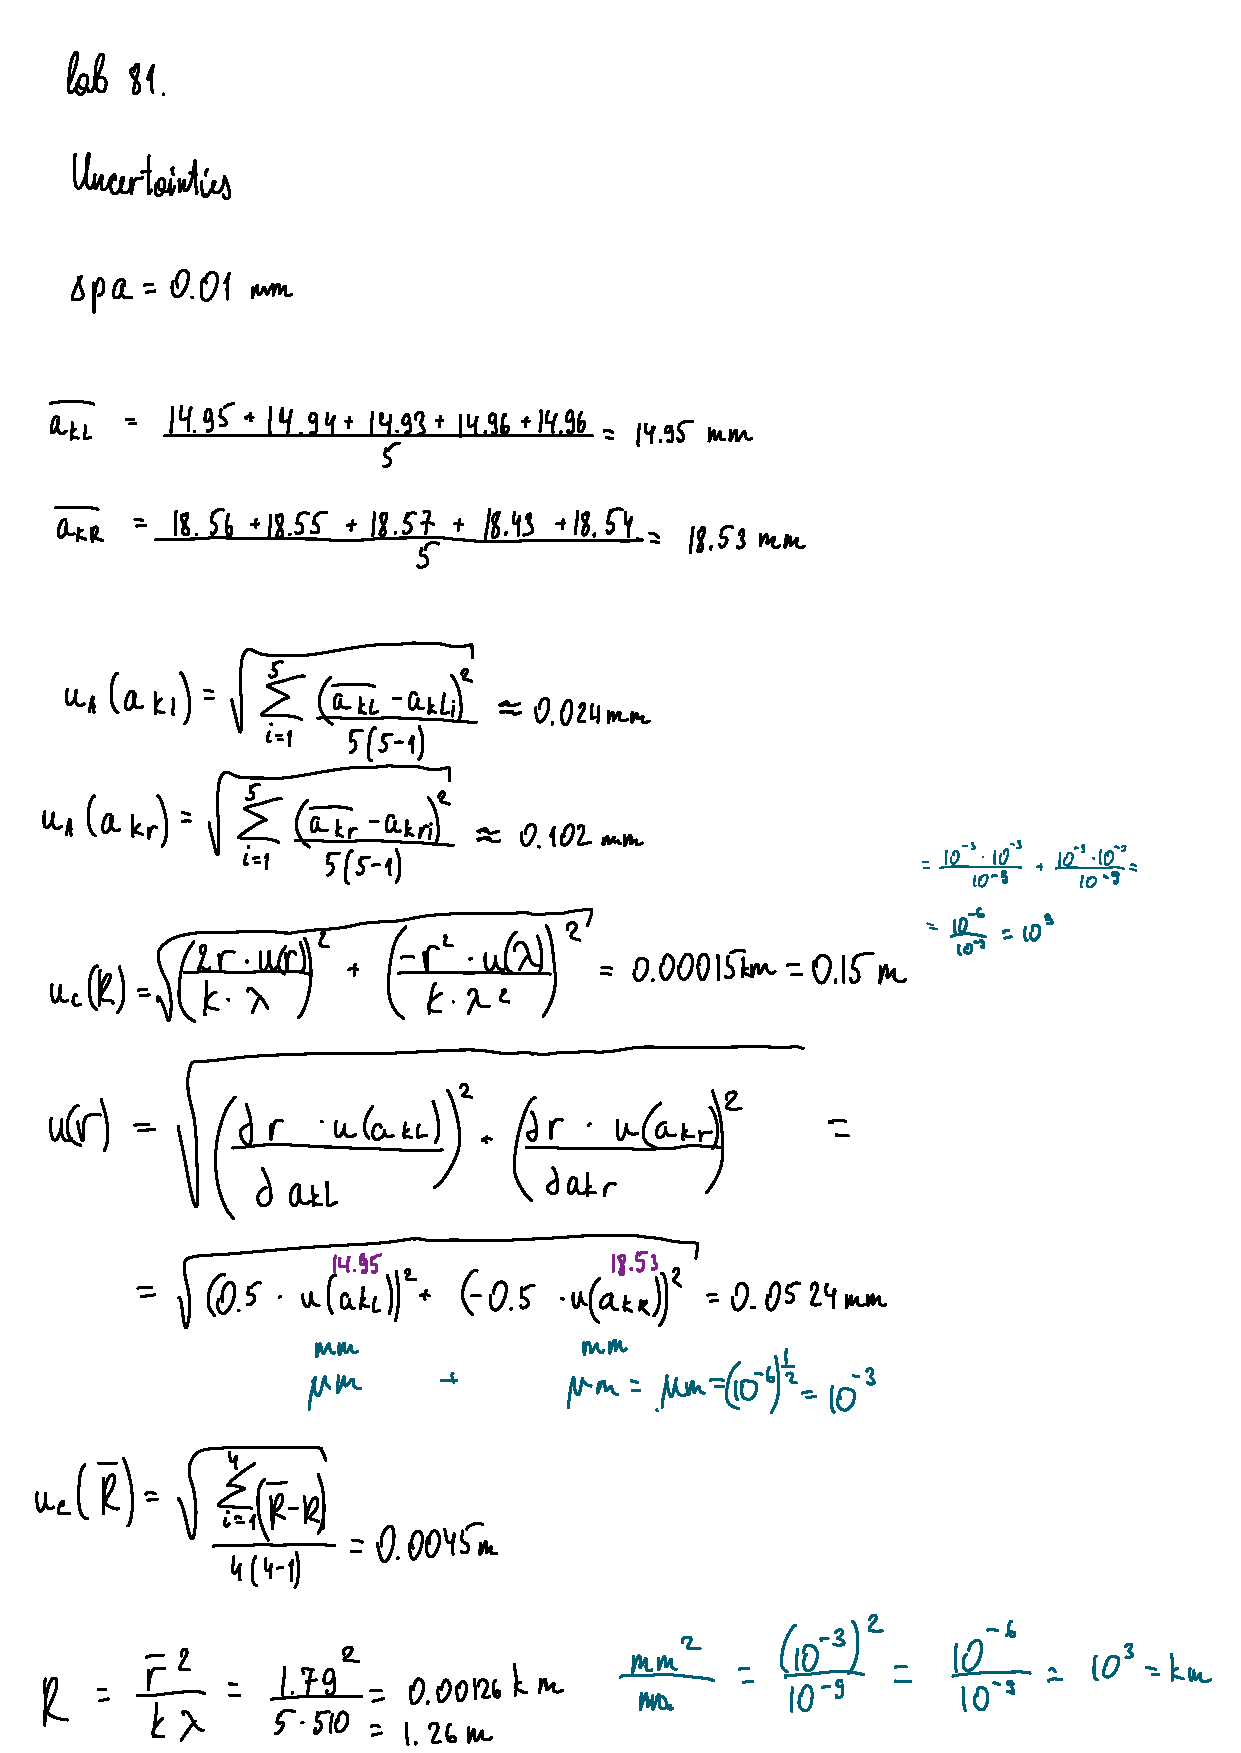
\includegraphics[width=10.8cm]{schematics/Calculations.pdf}
	\caption{Uncertainties and calculations }
\end{figure}
\begin{figure}[H]
	\centering
	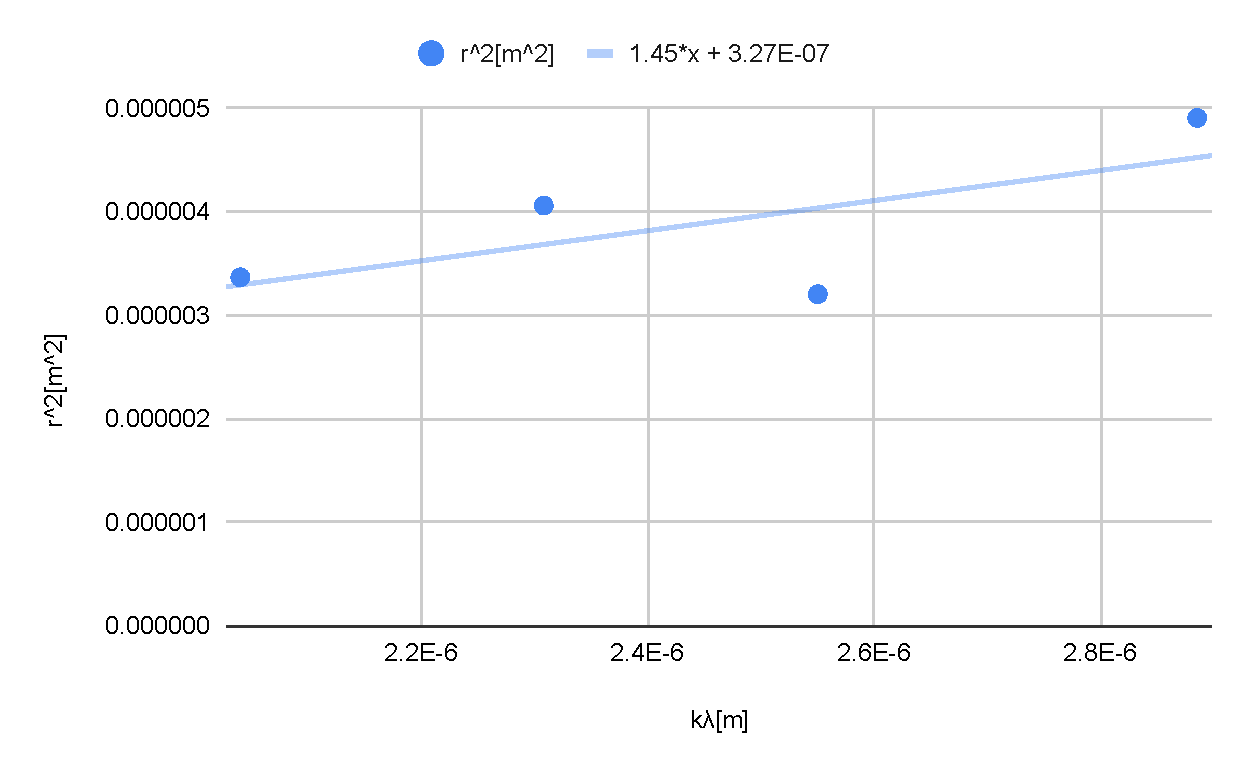
\includegraphics[width=10.8cm]{schematics/chart.pdf}
	\caption{graph of the squares of the determined ring's radii $r^2$ vs the product of sodium
light wavelength}
\end{figure}

\begin{table}[H]
    \centering
    \begin{tabular}{|l|l|}
    \hline
        R[m] & u(R)[m] \\ \hline
        1.45 & 0.4277 \\ \hline
    \end{tabular}
\end{table}














